
\toolName\  was developed as a  MATLAB~\cite{matlab} standalone application.
It is developed on top of an existing  planner presented in~\cite{tumova2016multi} which has been chosen since it already implements a decentralized planning procedure.
\toolName\ calls this planner twice considering two different versions of the model of the robots and their environments. 
The results obtained by performing this procedure are sound and correct.
Additional details and proofs can be found in~\cite{mapmaker17}.


\toolName\ can be executed in two ways, as shown in Listing~\ref{lst:command}.
\texttt{Scenario} is a Matlab file containing the model of the environment and the robots and \texttt{Experiment} encode the mission that must be satisfied by each robot.
The first option is the general way of executing the tool, using custom scenarios and experiments developed by the user.
In the second option the research question \texttt{RQ} that we tried to answer in this paper has to be specified.
This option is used for replicating the results that we present in~\cite{mapmaker17}.

\begin{lstlisting}[frame=single, backgroundcolor=\color{light-gray}, basicstyle=\footnotesize\ttfamily, language=Java, numbers=left, numberstyle=\tiny\color{black},caption= {Running \toolName}\label{lst:command}, captionpos=b]
mapmaker_exp 'Scenario', 'Experiment')
mapmaker_exp 'Scenario', 'Experiment', 'RQ')
\end{lstlisting}

%The tool is composed by several MATLAB-based scripts that can be executed independently for performing certain functions.
%In order to use \toolName it is sufficient to launch the function \emph{mapmaker\_exp} where the \emph{research question}, the \emph{example} or map of the environment and the \emph{experiment} to check are their arguments.
%This function enormously simplifies the performance of the tool, but there are other functionalities that can also be exploited explained in the previous section.





%In a normal case where the scenarios are already defined, the only components of the architecture depicted in~\ref{fig:overview} that are used are the \emph{Replication Package}, the \emph{Robot \& Environment models with uncertainty}, the \emph{Planner} itself and its inputs and, of course, the \emph{Solutions container}.
%The first component represents a folder where the models of the robot and environment with a certain added uncertainty for the selected experiment are stored.

When  \toolName\ is launched a graphical interface similar to the one presented  in Figure~\ref{fig:outputexample} is showed.
The grid represents the environment in which robot are moving.
Each cell represents a location of the environment and has a number associated, as labeled in some of them.
Robots are represented by the squared colored boxes.
Actions are used to encode movement, i.e., each robot can move left, right, up and down.
A robot  cannot move between adjacent cells if they are separated by thick bordered lines.
Whenever  it is unclear if a robot can move between adjacent cells, these cells are separated by a red border.
Each service is associated with a number.
Whenever a service can be provided by a robot in a cell, the cell is labeled with the corresponding number.
Finally, synchronization capabilities are represented by a black cross.
If it is unclear if two robots can synchronize in a cell, the cell is labeled with a green cross.
The graphical interface shows the plan execution.
Assume for example that the robots $r_1$, $r_2$ and $r_3$ have the following \emph{local missions}.
Robot $r_1$ has to perform the action 1, which is present in cells 7 and 9---note that the missions associated with each robot are colored with the color used for representing the robot.
Action 1 and action 2 (which has to be accomplished by robot $r_2$) are located in a cell labeled with a cross, so robot must meet there and perform both actions at the same time.
Robot $r_1$ can also perform this mission in cell 9, but it is unsure the synchronization in this cell.
As explained before, robot $r_2$ must synchronize with robot $r_1$ and perform action 2, but then it has to reach cell 22 for performing action 3.
Finally, robot $r_3$ has to perform action 4 in cell 2 and action 5, which can be possibly executed in cell 18 or in cell 30.

In figure~\ref{fig:outputexample} we represented different plans performed by the robots. 
Starting from robot $r_1$, there are two different plans that could be performed.
P1 represents a definitive plan and P1' a possible plan where a true evidence was detected by the robot.
In those paths the robot basically reaches the cell where the action can be performed with the help of robot $r_2$ and moves away. 
In both cases the plan is repeated continuously.
For robot $r_2$ we represented two different paths as well.
P2 represents a possible plan ---due to the uncertainty of the door between cells 14 and 20--- where $r_2$ synchronizes with $r_1$ in order to accomplish action 2.
P2' is a similar path with the difference that the synchronization is performed in cell 9, where the it is uncertain.
In both cases the plan is repeated continuously.
Finally, P3 represents a possible path where robot $r_3$ accomplishes action 4 and then action 5 in cell 18.
Then, it performs the same action continuously.
\sergio{label paths in the picture}
We produced a video that shows how to execute the tool and its performance. 
It is available in~\footnote{https://goo.gl/jYeLbm}.

%The results achieved and presented in~\cite{mapmaker17} can be replicated using this models.
%They are loaded and set as MATLAB workspace variables in the second component.

%The planner needs as input the information from this variables and also from the scripts \emph{Algorithms}, \emph{Utils} and \emph{Configuration files}, that are automatically linked.
%During the execution of the planner \sergio{image representing the execution of the tool?} the MATLAB interface shows a window with the goals of the current mission. 
%Furthermore, after the computation of the plan it shows the movements of the robots and their knowledge of the environment.
%When all the robots have reached their goals or they realized that their local mission is not feasible the experiments concludes.
%Once the experiment is concluded, the data extracted (as explained in~\ref{sec:approach}) is stored in the solutions container component.


\begin{figure}[t]
\begin{center}
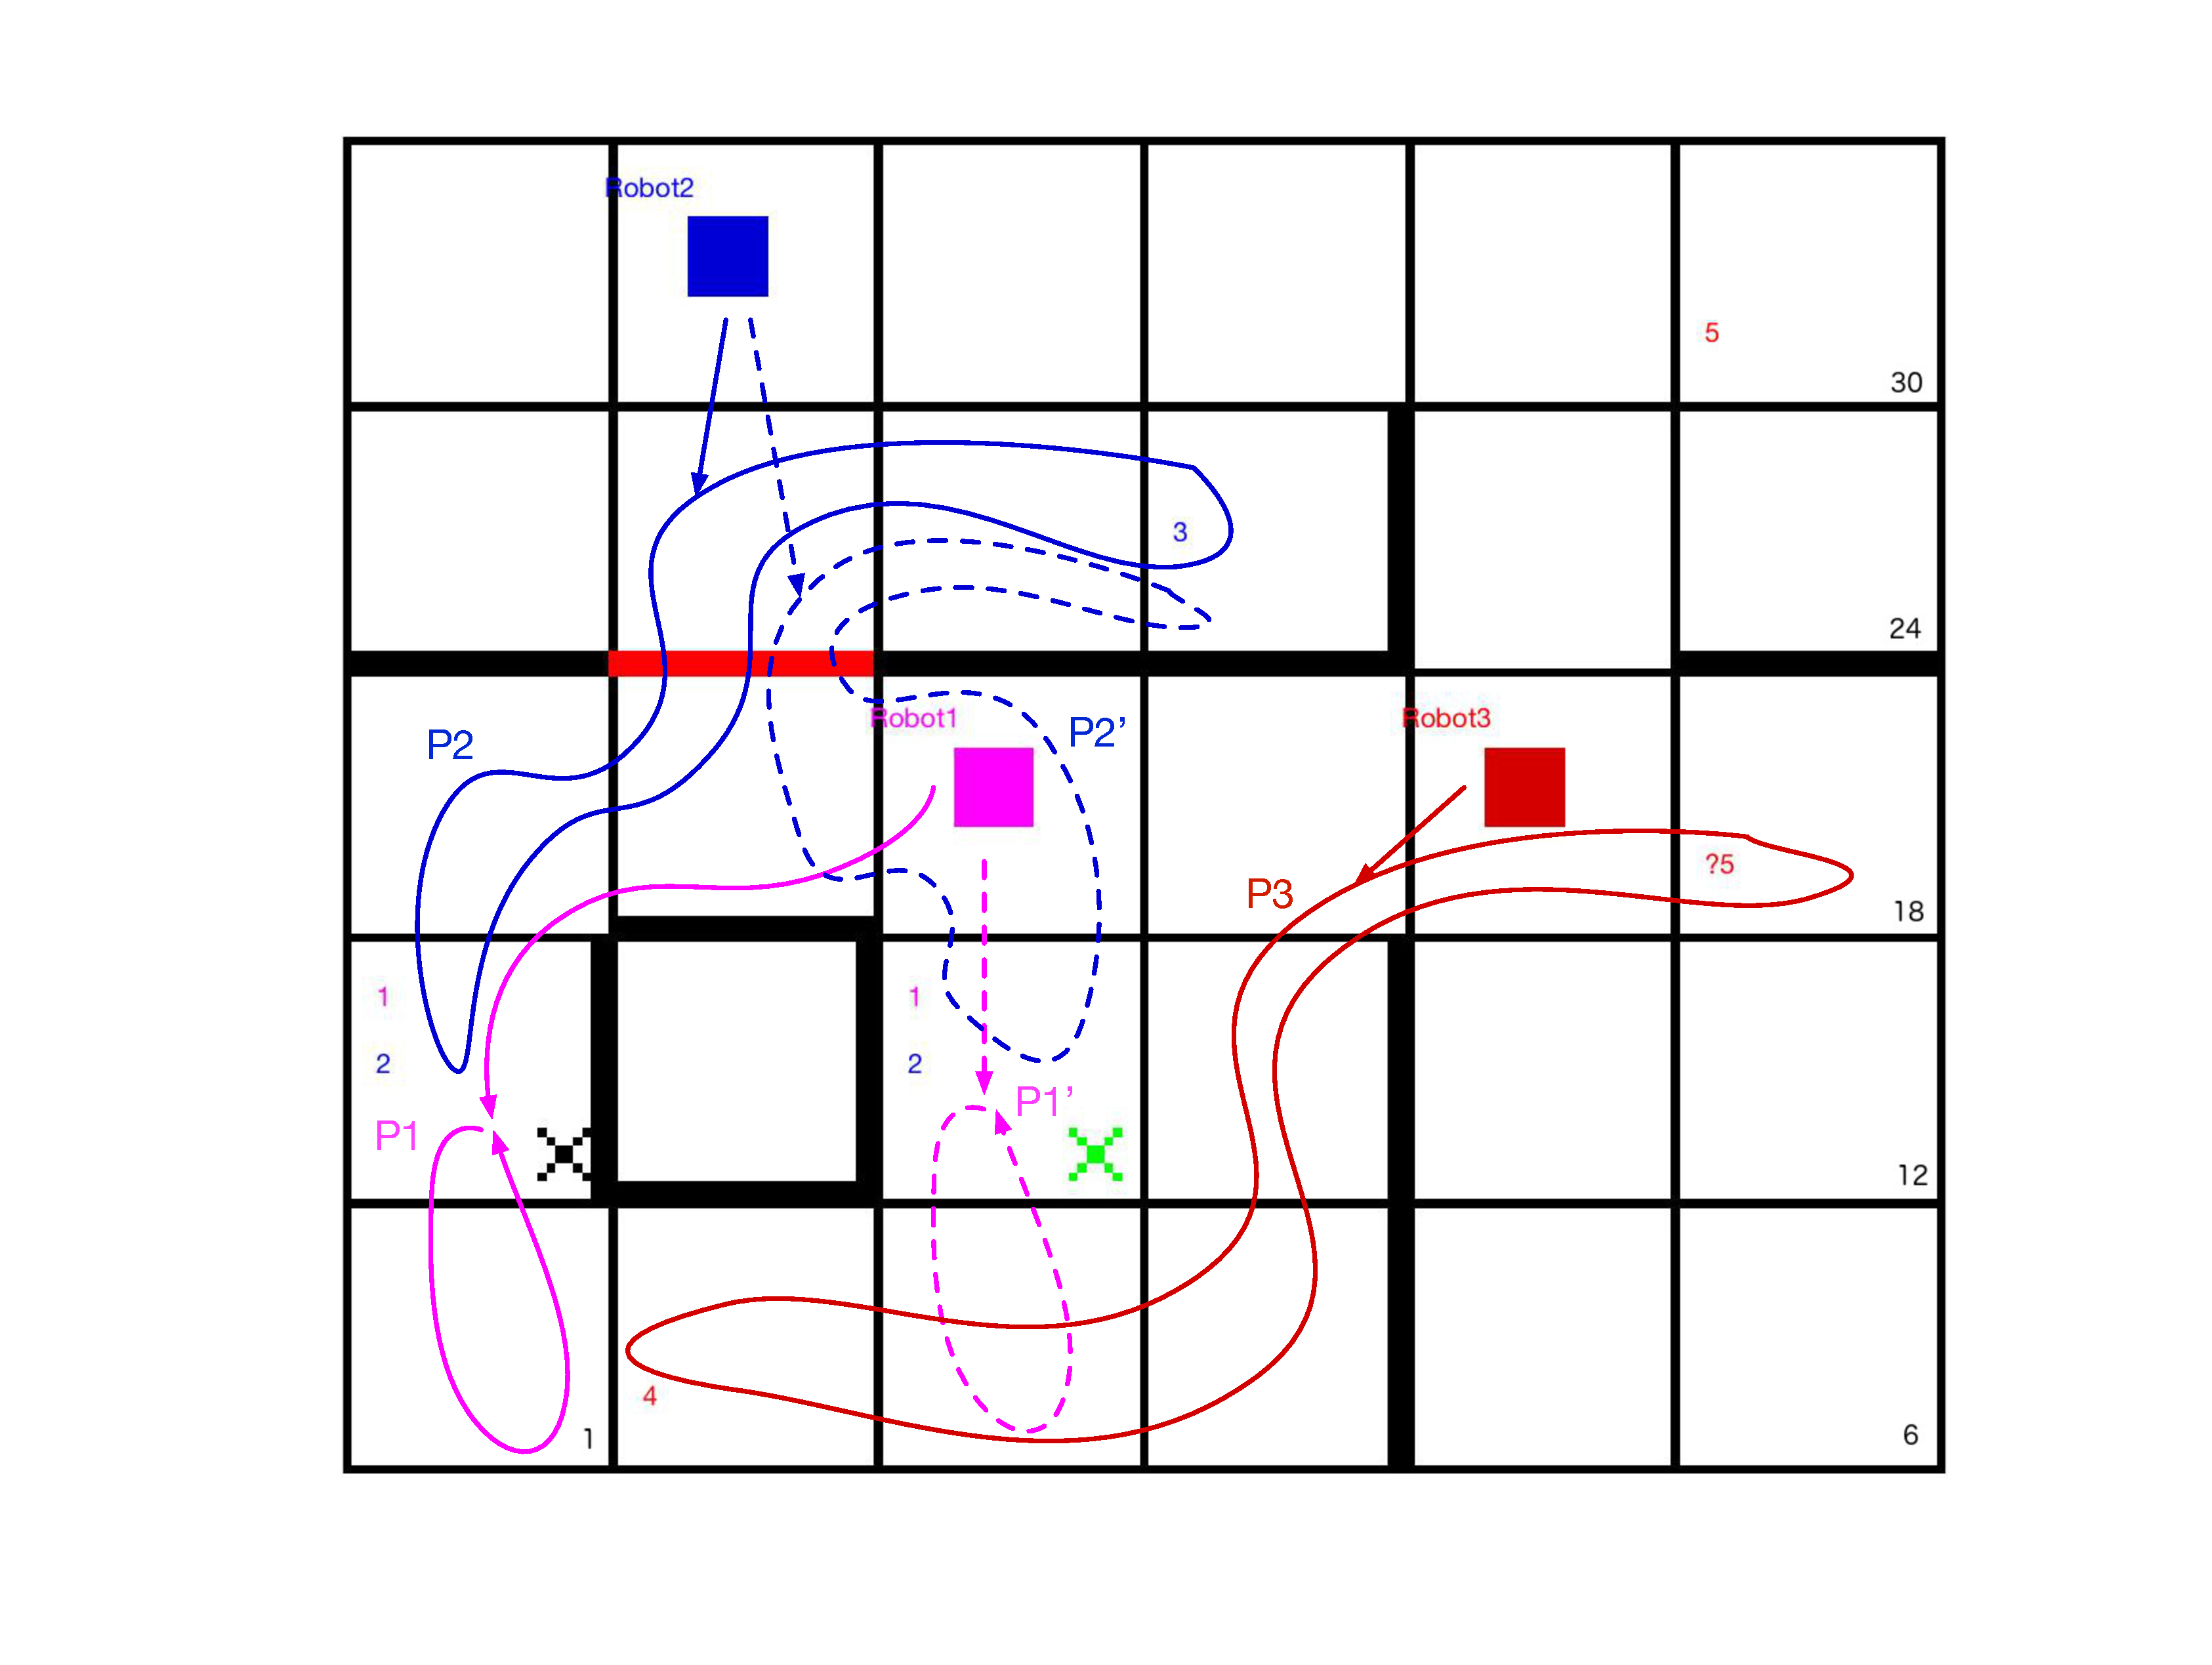
\includegraphics[width=1\linewidth]{Figures/arrows.pdf}
\caption{\toolName\ usage scenario.}
\label{fig:outputexample}
\end{center}
\end{figure}

%In~\cite{mapmaker17}  we have shown that our tool is able to perform a plan even in environments full of uncertainty.
%Thus, \toolName~ is able to compute a plan where other planners will not.
%However, the computation time and the number of actions to be performed by the robot that tries to follow a possible plan and detects a false evidence are normally greatly increased.
%This increasing is due to required re-computing that has to be performed when looking for a new possible plan.

%For checking its performance the tool was tested in different environments based on real-world scenarios.
%The model of the uncertainty of the environment was randomly created and matched with randomly models of the robots (service and synchronization locations and uncertainties).
%The performance of tool was evaluated in two Research Questions divided in three experiments (one for each kind of uncertainty defined for this project).
%The results are presented and discussed in~\cite{mapmaker17}.

%\textbf{Tool Validation}


